\section{Desarrollo}

\subsection{PARTE I: Instalación Hyper-V}

\textbf {4.1.1. Verificar Edición de Windows 10:} El Hyper V es una característica de Windows 10 en las versiones PRO y Educational, para esto primero verificaremos si nuestro sistema pertenece a alguna de esas ediciones.
\begin{center}
  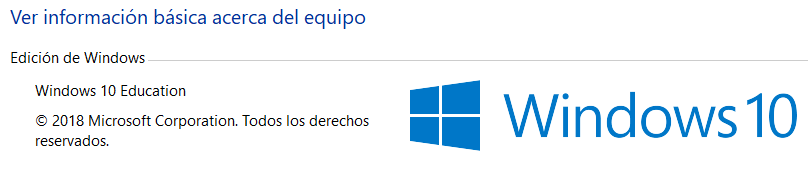
\includegraphics[width=15cm]{Imagenes/Windows_Education.png}
\end{center}

\textbf {4.1.2. Buscar la opción de Características de Windows:} Nos dirigimos al Menu del Windows 10 y buscamos la opción de "Activar o desactivar las caracterísitcas de Windows".\\
\begin{center}
  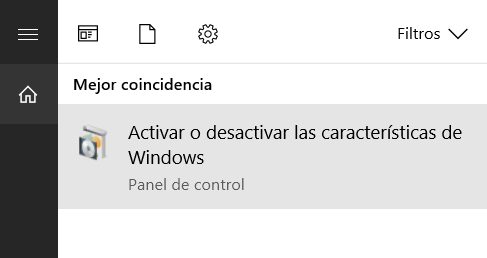
\includegraphics[width=15cm]{Imagenes/Activar_Caracteristicas.png}
\end{center}
\break

\textbf {4.1.3. Activar Característica Hyper-V:} Buscamos la opción llamada "Hyper V" y lo activamos.\\
\begin{center}
  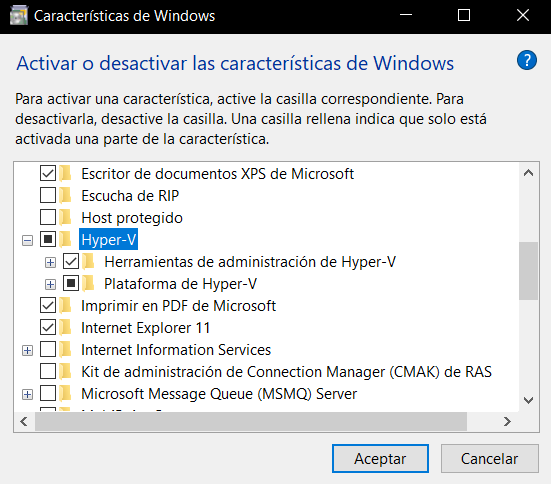
\includegraphics[width=11cm]{Imagenes/Activar_Hyper_V.png}
\end{center}

\textbf {4.1.4. Reiniciar el Sistema Operativo:} Con la finalidad de que se apliquen los cambios, es necesario reiniciar el equipo.
\begin{center}
  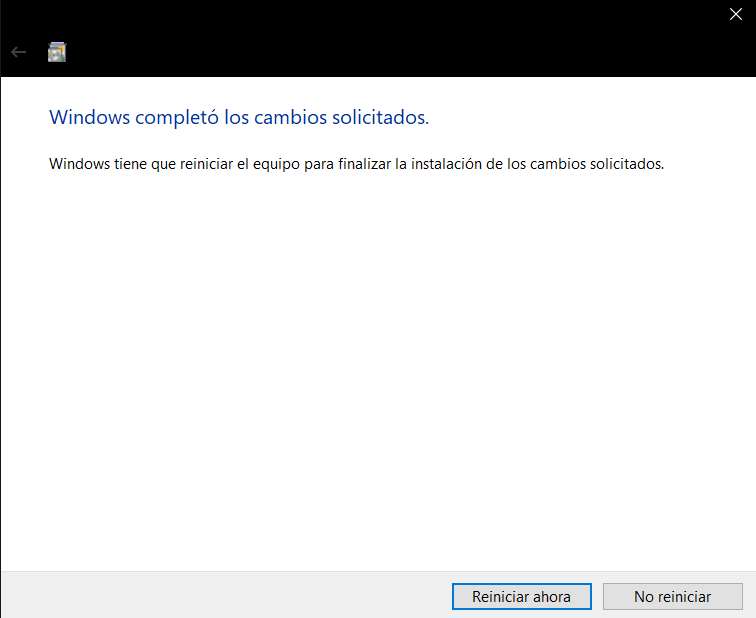
\includegraphics[width=11cm]{Imagenes/Reiniciar.png}
\end{center}
\break

\textbf {4.1.5. Hyper V correctamente habilitado:} Una vez reiniciada la computadora, ya podremos abrir nuestro Hyper-V que estará listo para ser configurada.\\
\begin{center}
  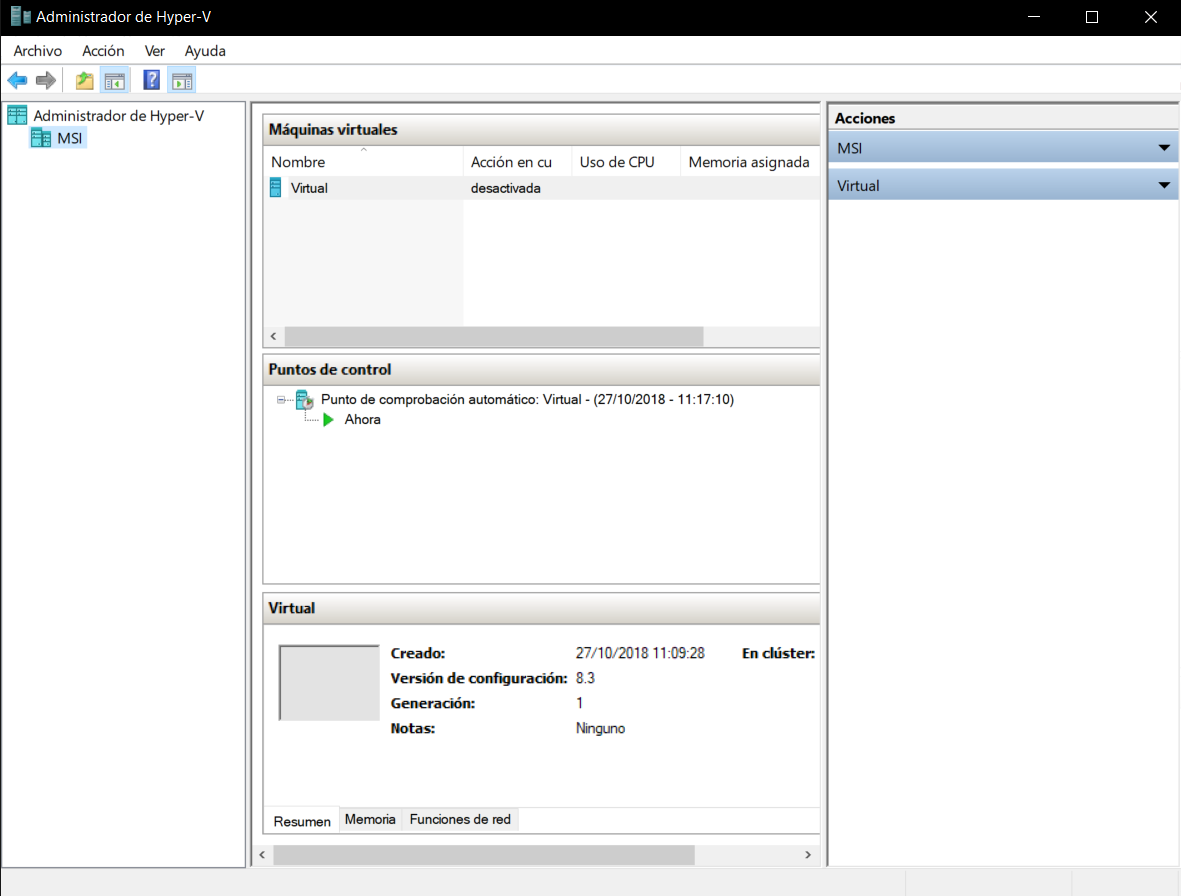
\includegraphics[width=14cm]{Imagenes/Hyper_V.png}
\end{center}
\break

\subsection{PARTE II: Instalación Windows Server 2016}

\textbf {4.2.1. Crear Nueva maquina Virtual:} En este paso crearemos una nueva maquina virtual donde instalaremos nuestro Windows Server 2016, para eso le daremos clic derecho a nuestro servidor de HYPER V.
\begin{center}
  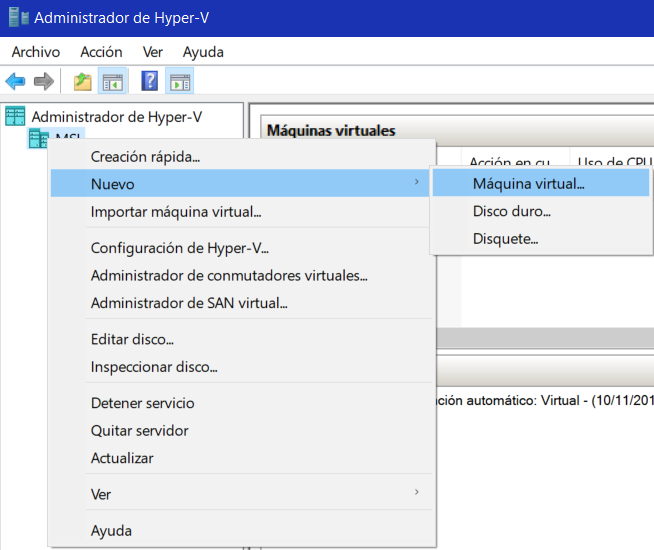
\includegraphics[width=11cm]{Imagenes/Nueva_Maquina.png}
\end{center}

\textbf {4.2.2. Especificar Nombre:} Ahora especificaremos el nombre de nuestra maquina virtual, en este caso le colocaremos Windows Server 2016.
\begin{center}
  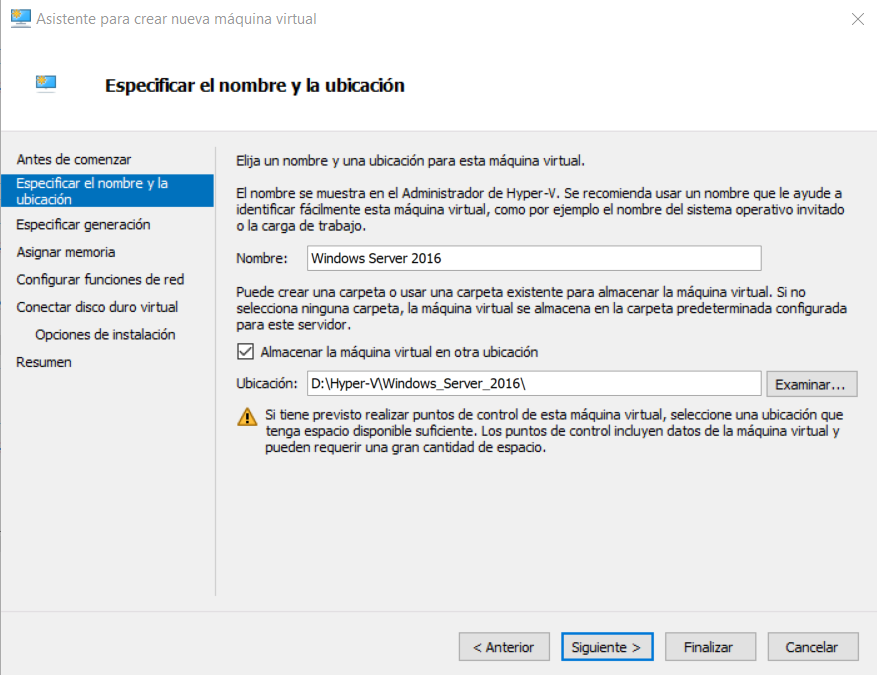
\includegraphics[width=11cm]{Imagenes/Especificar_Nombre_Ruta.png}
\end{center}
\break

\textbf {4.2.3. Elegir Generación:} Elegiremos la Generación que se marca por defecto, en este caso es la Generación 1.
\begin{center}
  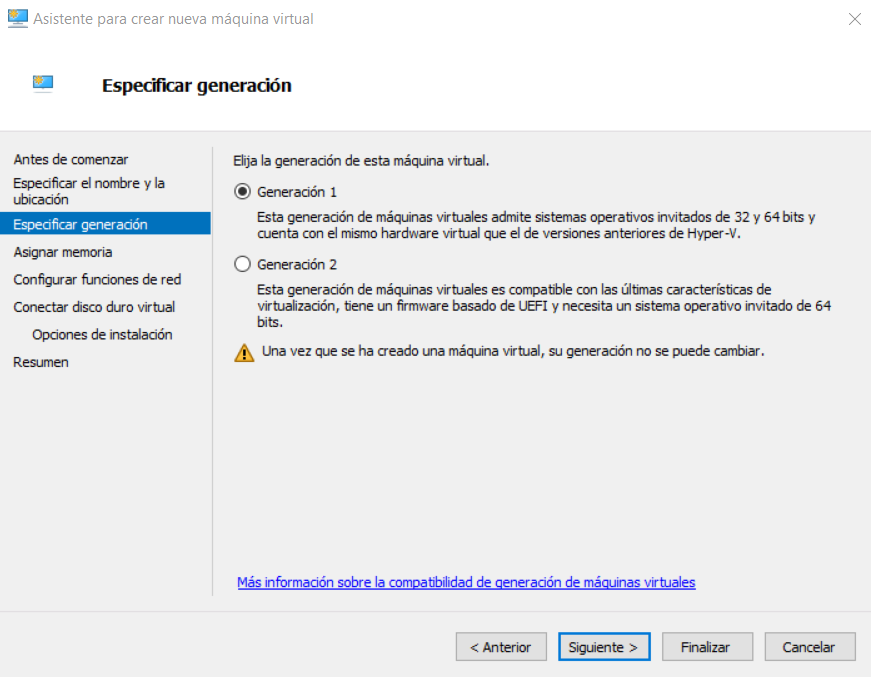
\includegraphics[width=11cm]{Imagenes/Especificar_Generacion.png}
\end{center}

\textbf {4.2.4. Asignar Memoria:} Elegiremos la cantidad de memoria con la que queremos que trabaje nuestra maquina virtual, en este caso le pusimos 2048mb y le damos clic en Siguiente.
\begin{center}
  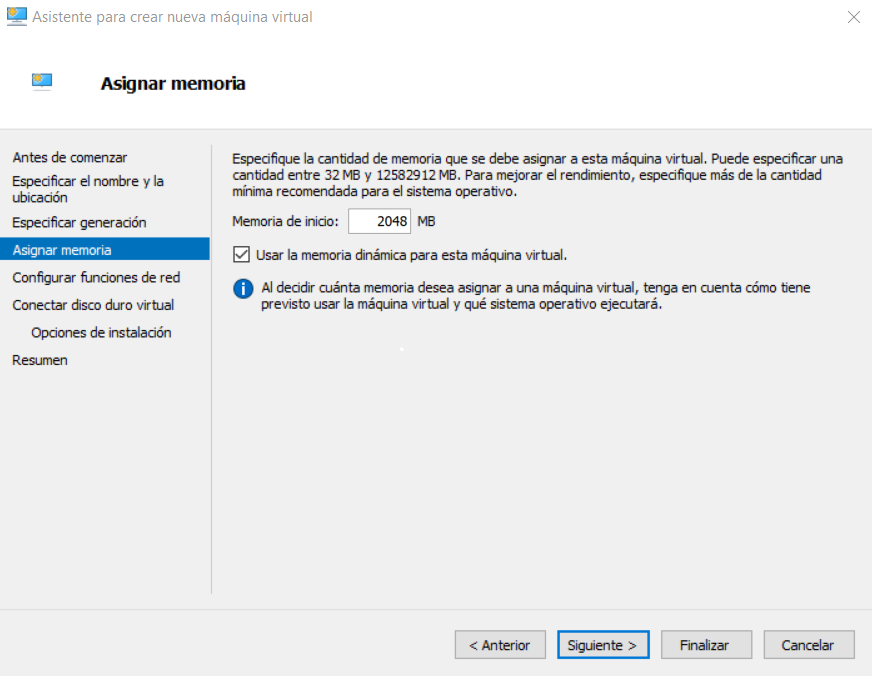
\includegraphics[width=11cm]{Imagenes/Asignar_Memoria.png}
\end{center}
\break

\textbf {4.2.5. Conectar Disco:} Estableceremos la ruta de nuestra maquina virtual y le asignaremos el tamaño de 80GB.
\begin{center}
  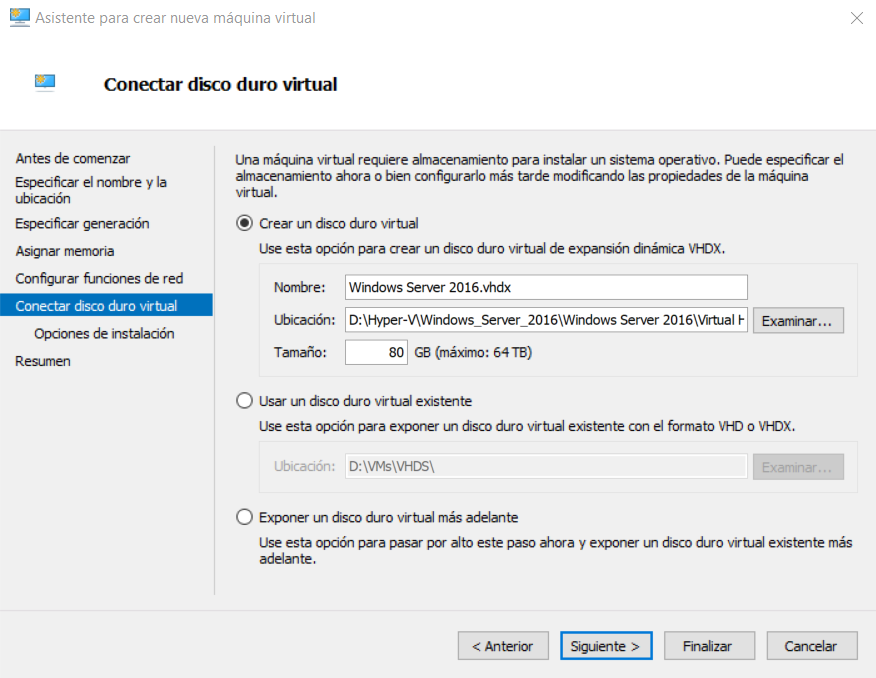
\includegraphics[width=11cm]{Imagenes/Conectar_Disco.png}
\end{center}

\textbf {4.2.6. Resumen:} Al terminar con la configuración, el asistente nos mostrará un Resumen de nuestra máquina virtual, si todo esta conforme le daremos clic en FINALIZAR.
\begin{center}
  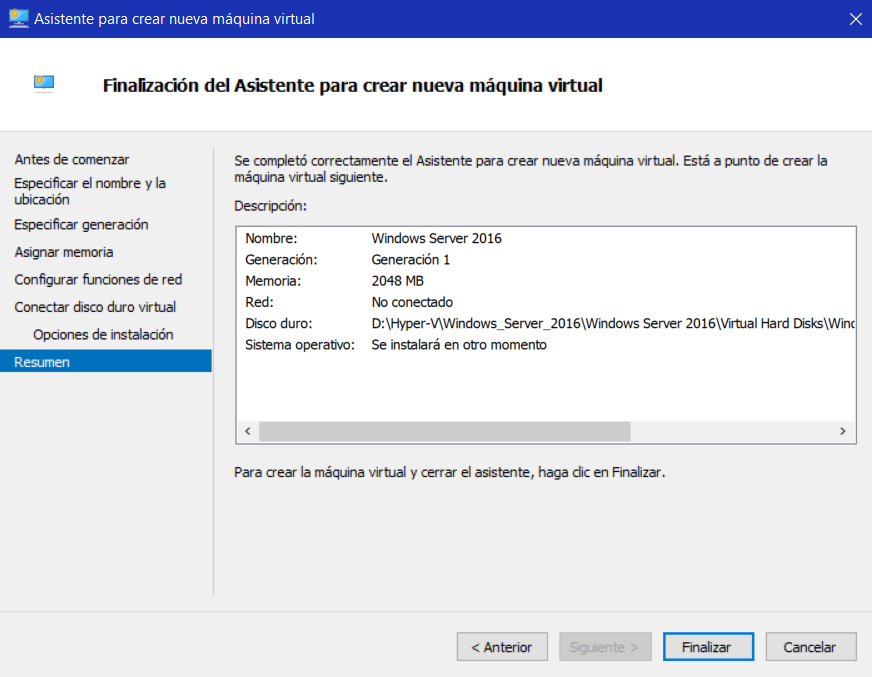
\includegraphics[width=11cm]{Imagenes/Resumen.png}
\end{center}
\break

\textbf {4.2.7. Conectar con la Máquina Virtual:}Para este paso le daremos clic derecho sobre nuestra máquina virtual y le damos clic en Conectar.
\begin{center}
  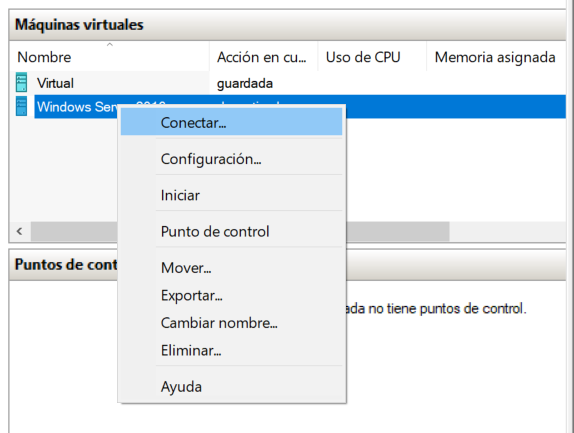
\includegraphics[width=11cm]{Imagenes/Conectar_WindowsServer.png}
\end{center}

\textbf {4.2.8. Iniciar Virtualización:} Una vez que hayamos conectado nuestra máquina virtual, se nos abrirá el virtualizador, nosotros le daremos clic en INICIAR, para que comience a virtualizar.
\begin{center}
  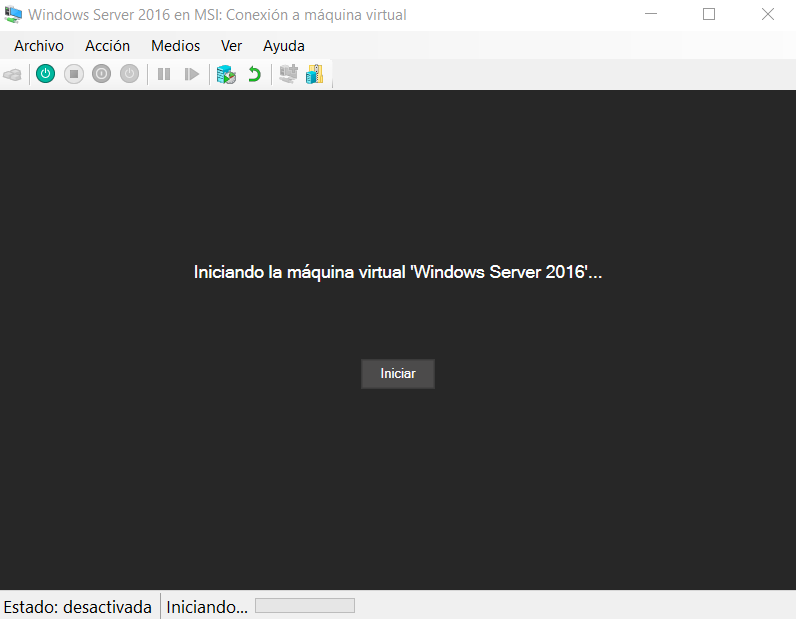
\includegraphics[width=11cm]{Imagenes/Iniciar_Virtualizacion.png}
\end{center}
\break

\textbf {4.2.9. Elegir el ISO de instalación:}Para este paso le daremos clic en Medios - Unidad de DVD y seleccionaremos la nuestro ISO.
\begin{center}
  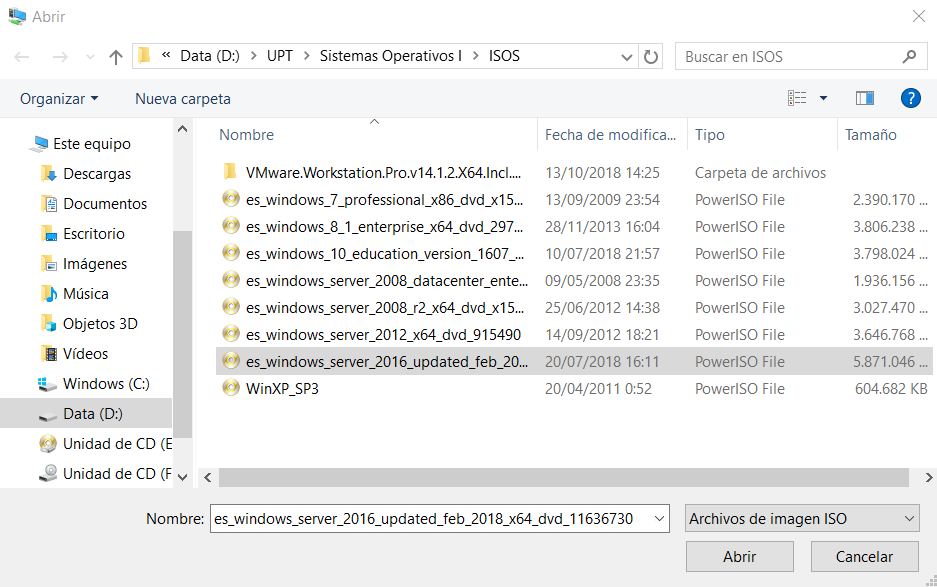
\includegraphics[width=11cm]{Imagenes/Elegir_ISO.png}
\end{center}

\textbf {4.2.10. Iniciar Instalación:} Luego de elegir nuestro ISO, volveremos a Iniciar nuestra Virtualización seguidamente nos aparecerá el cuadro de Instalación de Windows Server.
\begin{center}
  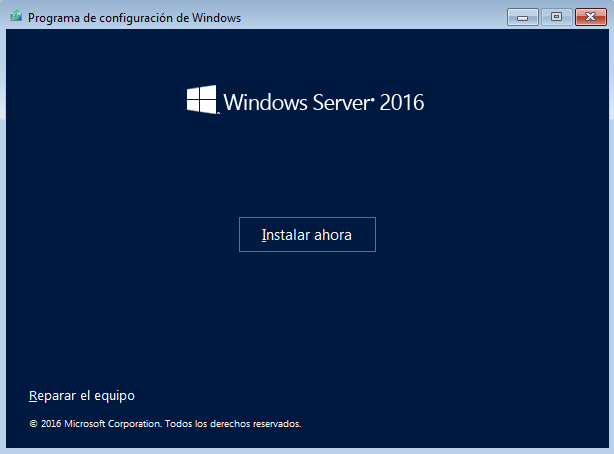
\includegraphics[width=11cm]{Imagenes/Instalar_Ahora.png}
\end{center}
\break

\textbf {4.2.11. Configuración de la Instalación:} Luego de hacer clic en Instalar Ahora, nos aparecera un cuadro donde podremos elegir el tipo de Idioma que deseamos usar en nuestro Windows Server, nosotros elegiremos Español Perú y le daremos clic en Siguiente.
\begin{center}
  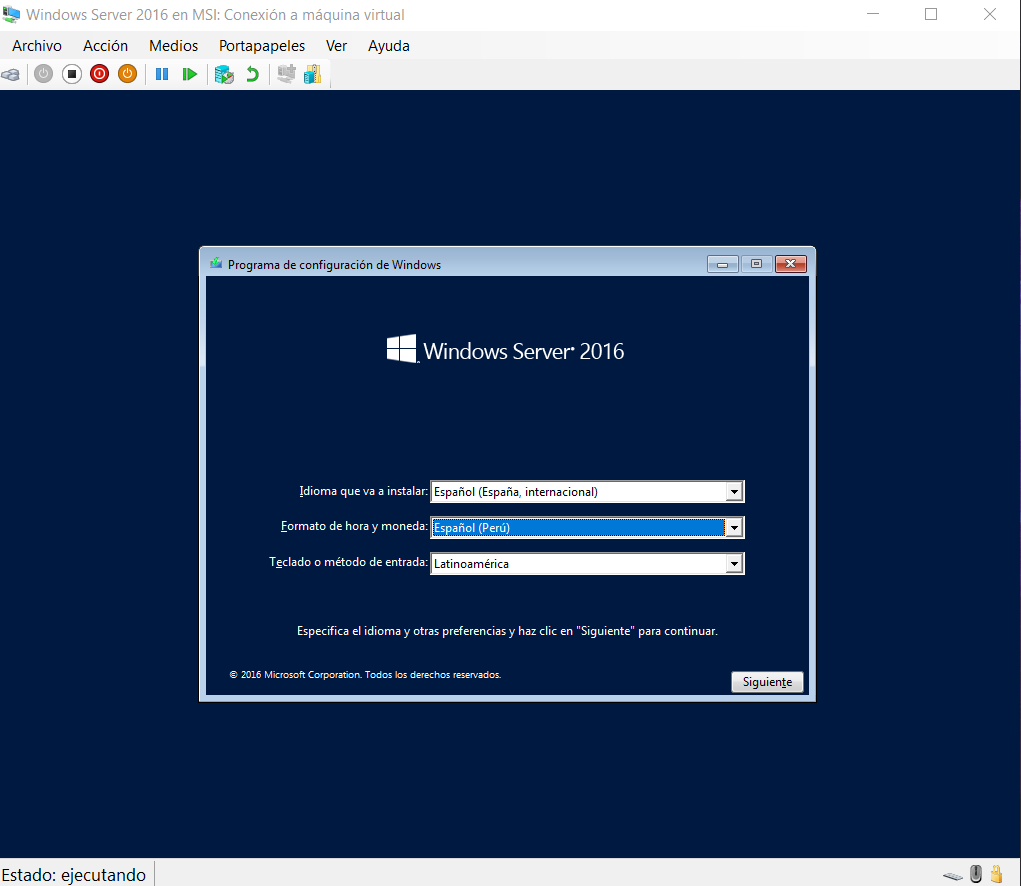
\includegraphics[width=11cm]{Imagenes/Iniciar_Instalacion.png}
\end{center}

\textbf {4.2.12. Ingresar Serial:} Si hemos comprado el software, debemos ingresar el Serial que llega junto al Instalador, en caso de no tener el Serial le damos clic en la opción: No tengo Clave del Producto y Siguiente.
\begin{center}
  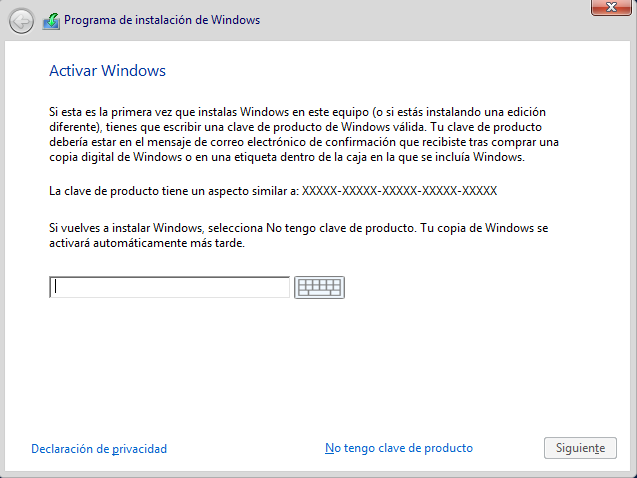
\includegraphics[width=11cm]{Imagenes/Ingresar_Serial.png}
\end{center}
\break

\textbf {4.2.13. Elegir Versión:} Elegiremos la opción de Windows Server 2016 DataCenter (Experiencia de Escritorio) y le damos clic en Siguiente
\begin{center}
  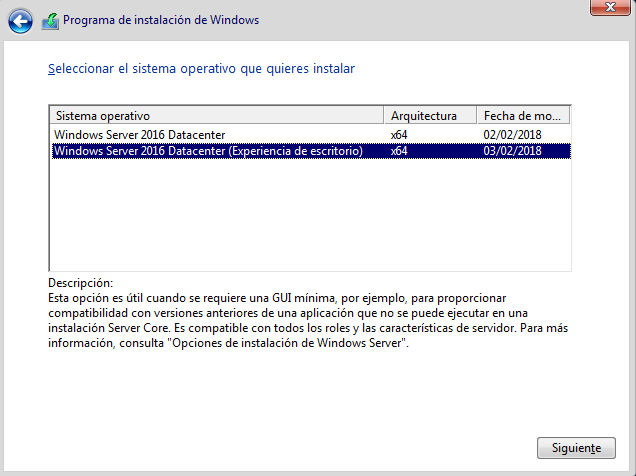
\includegraphics[width=11cm]{Imagenes/Elegir_Version.png}
\end{center}

\textbf {4.2.14. Aceptar Licencia:} Leeremos los términos y licencia y activaremos el check de ACEPTO, y luego clic en Siguiente.
\begin{center}
  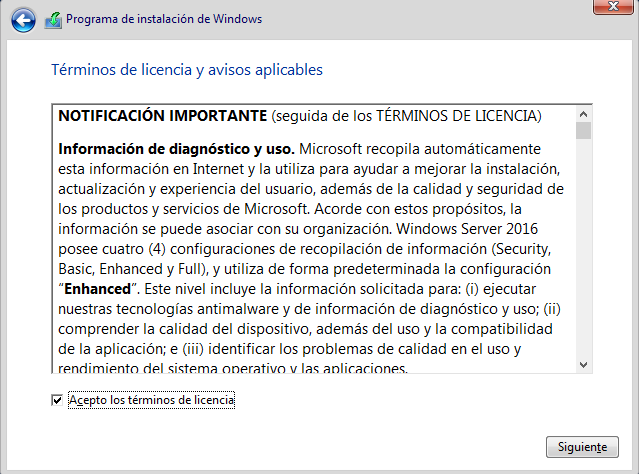
\includegraphics[width=11cm]{Imagenes/Aceptar_Licencia.png}
\end{center}
\break

\textbf {4.2.15. Tipo de Instalación:} Nosotros le daremos clic en Instalación Personalizada.
\begin{center}
  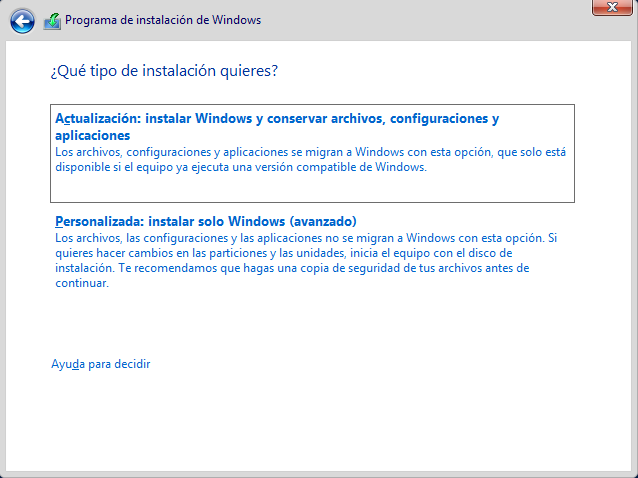
\includegraphics[width=11cm]{Imagenes/Elegir_Tipo_Instalacion.png}
\end{center}

\textbf {4.2.16. Disco de Instalación:} Elegiremos el único disco disponible (Unidad 0) y le daremos clic en Siguiente.
\begin{center}
  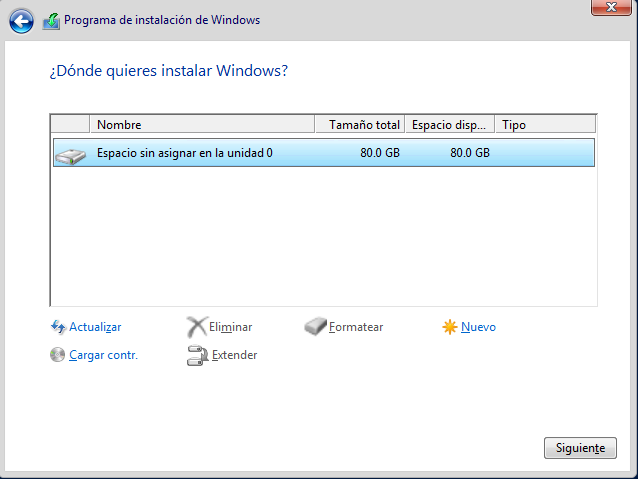
\includegraphics[width=11cm]{Imagenes/Elegir_Disco_Instalacion.png}
\end{center}
\break

\textbf {4.2.17. Proceso de Instalacion:} Luego comenzará la Instalación de nuestro Windows Server, en este paso solo queda esperar a que la Instalación termine.
\begin{center}
  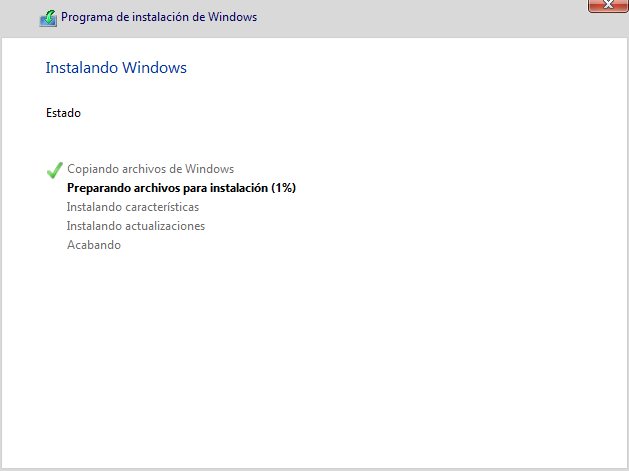
\includegraphics[width=11cm]{Imagenes/Proceso_Instalacion.png}
\end{center}

\textbf {4.2.18. Crear Clave:} Luego de que el Proceso de Instalación haya terminado, ahora debemos crear una clave para el Administrador del Servidor, en este caso nosotros le asignaremos la clave de: Sistemas.2018
\begin{center}
  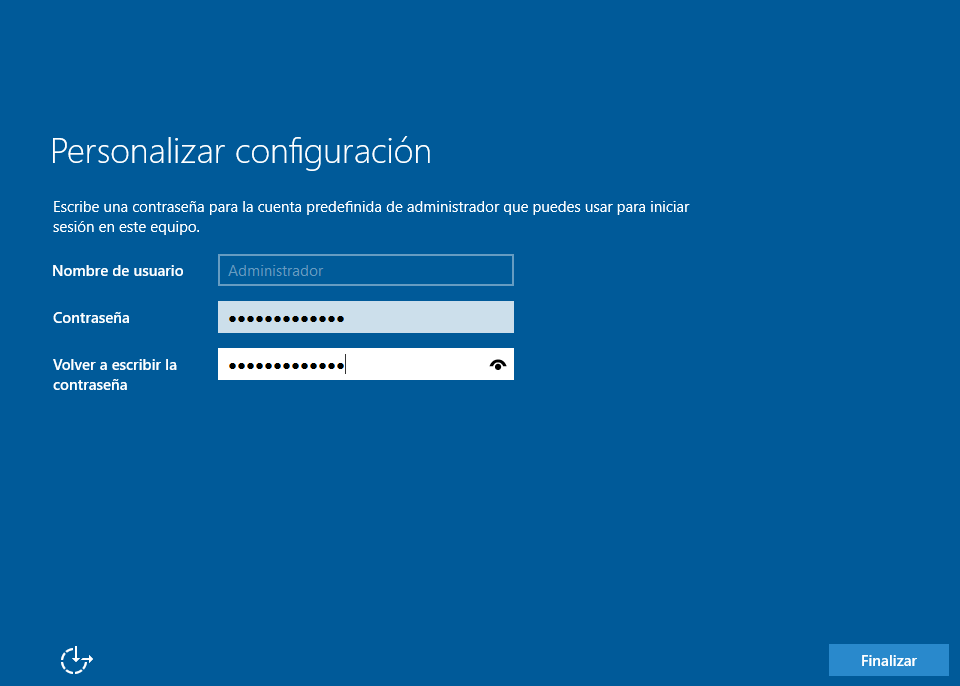
\includegraphics[width=11cm]{Imagenes/Crear_Clave.png}
\end{center}
\break

\textbf {4.2.19. Identificarse en el Windows Server:} En este paso debemos identificarnos para poder iniciar nuestro Windows Server, para esto ingresaremos con la contraseña antes creada: Sistemas.2018
\begin{center}
  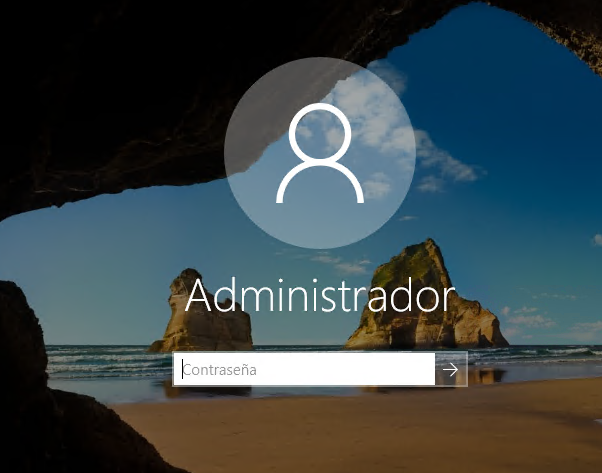
\includegraphics[width=11cm]{Imagenes/Identificarse.png}
\end{center}

\textbf {4.2.20. Windows Server 2016:} Luego de tanta espera, al fin podremos acceder a nuestro Windows Server la cuál se encuentra lista para poder instalarle el Oracle DataBase.
\begin{center}
  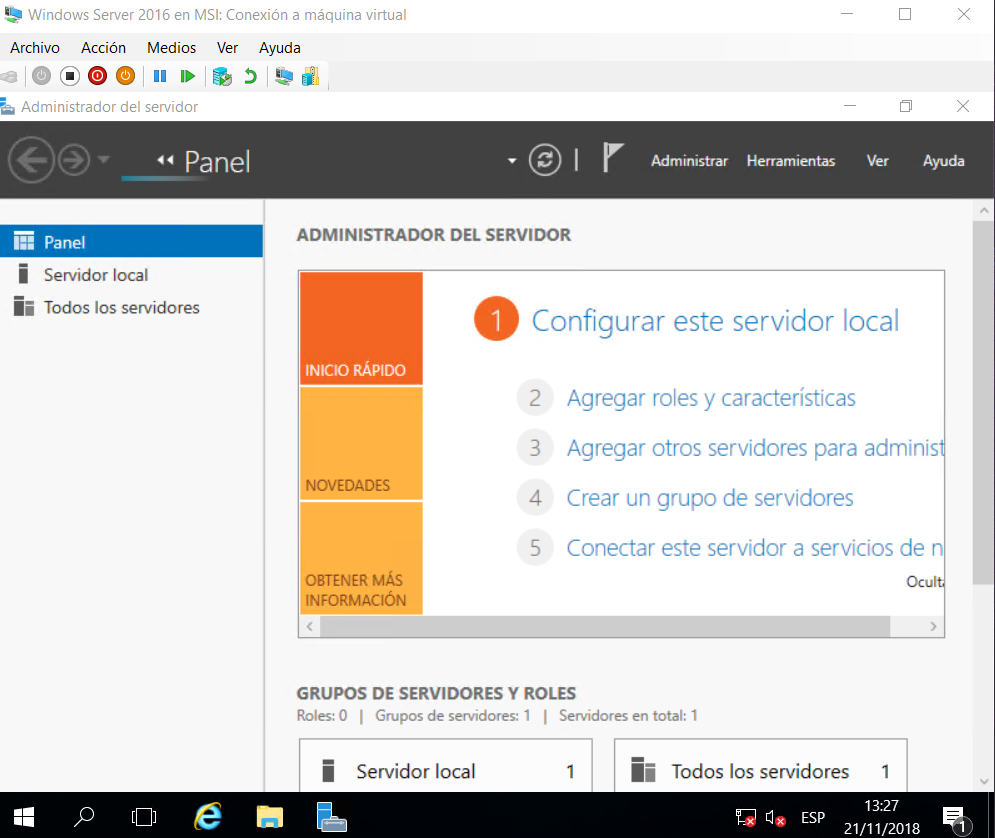
\includegraphics[width=11cm]{Imagenes/Escritorio_Windows_Server.png}
\end{center}
\break

\subsection{PARTE III: Instalación Windows Server 2016}

\textbf {4.3.1. Configuración antes de la Instalación:} Como primer paso configuraremos el archivo host que se encuentra en el Disco Local C
Usar las líneas 1 a 3 cuando se está utilizando una dirección IP de DHCP, y las líneas 1 a 4 cuando se está usando una dirección IP estática.  El nombre de hosts debe estar en minúscula. \\
Crear una cuenta de usuario  que no tenga espacio en blanco en el nombre por ejemplo jsequeiros, y conceder los privilegios de Administrador.
\begin{center}
  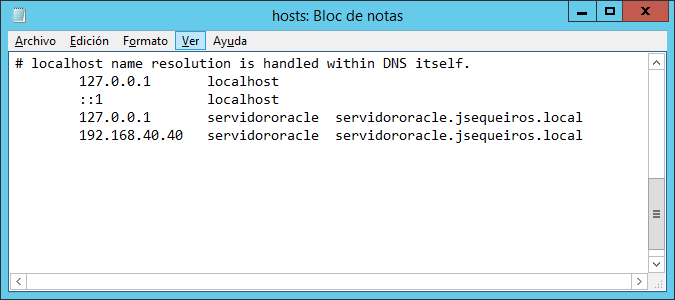
\includegraphics[width=12cm]{Imagenes/Configuracion_Host.png}
\end{center}

\textbf {4.3.2. Descargar el Instalador de Oracle Database:} Luego de la configuración del archivo hosts pasaremos a descargar nuestro Instalador, pasa eso nos dirigiremos a la pagina de www.oracle.com y descargaremos el Oracle Database para Microsoft Windows x64 (64-bit).
\begin{center}
  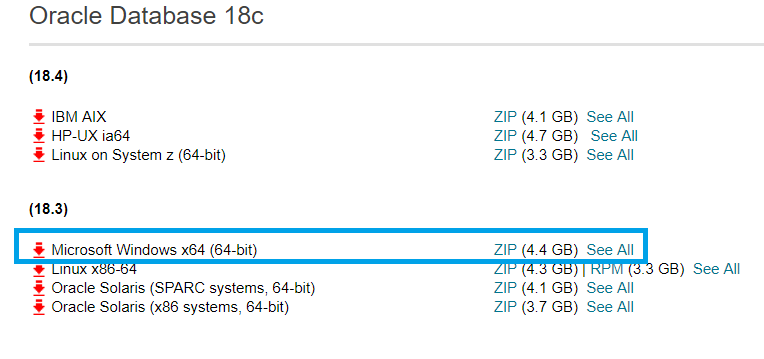
\includegraphics[width=12cm]{Imagenes/Web_Descarga_Oracle.png}
\end{center}
\break

\textbf {4.3.3. Descomprimir el Instalador:} Luego de descargar el Instalador, pasaremos a descomprimirlo, luego de hacerlo nos quedará de la siguiente forma:
\begin{center}
  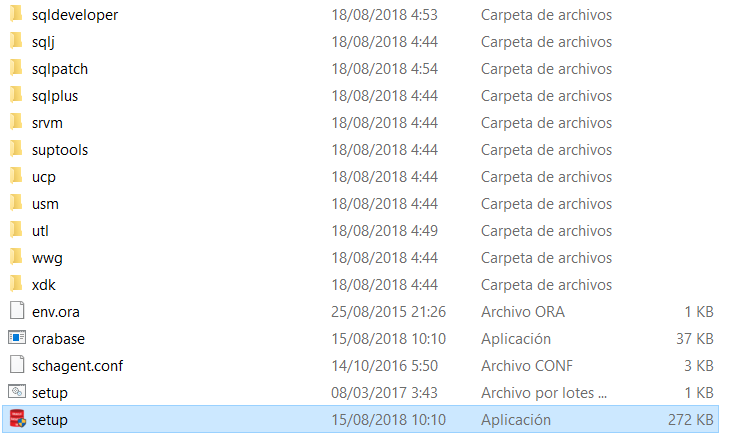
\includegraphics[width=12cm]{Imagenes/Descomprimir.png}
\end{center}

\textbf {4.3.4. Descomprimir el Instalador:} Dentro de la carpeta de instalación, ejecutar el archivo setup.exe y se abrirá la ventana del  Oracle Universal Installer, que puede permanecer unos segundos.
\begin{center}
  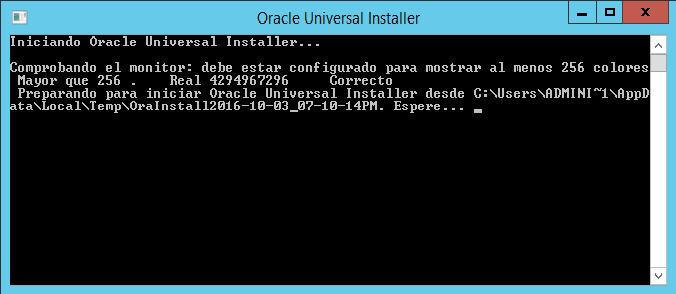
\includegraphics[width=12cm]{Imagenes/Instalador_Universal.png}
\end{center}
\break

\textbf {4.3.5. Configurar Actualizaciones:} En la siguiente pantalla pide proporcionar una dirección de correo electrónico para recibir información sobre los problemas de seguridad.  En este caso desactivamos la casilla de recibir actualizaciones de seguridad a través del soporte de Oracle.  Saldrá una ventana de notificación indicando que no se ha ingresado ninguna dirección de correo electrónico.  Clic en el botón si para continuar con la instalación.
\begin{center}
  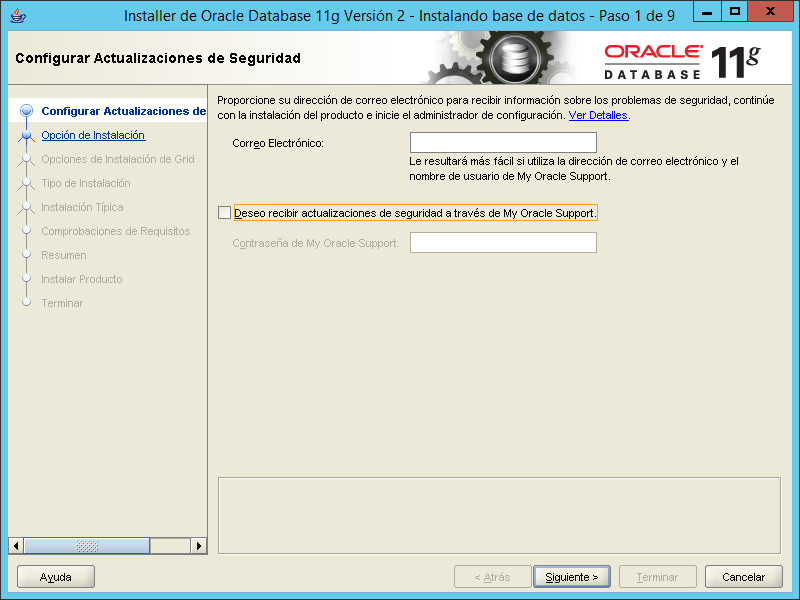
\includegraphics[width=12cm]{Imagenes/Configurar_Actualizaciones.png}
\end{center}

\textbf {4.3.6. Crear Base de datos:} Elegiremos la opción de Crear y Configurar Base de Datos y le daremos clic en Siguiente.
\begin{center}
  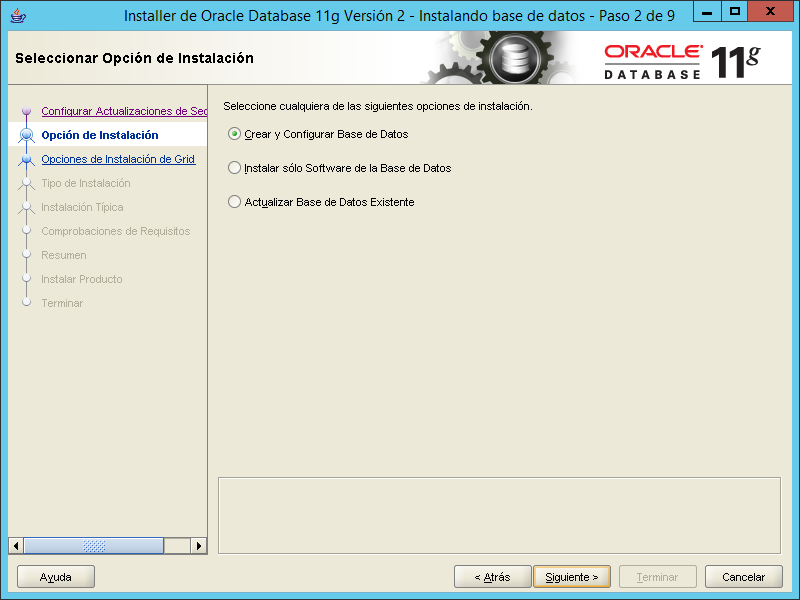
\includegraphics[width=12cm]{Imagenes/Opcion_Crear_Base.png}
\end{center}
\break

\textbf {4.3.7. Clase Escritorio:} Seleccionar "Clase de Escritorio", que es una instalación bastante más sencilla pues el asistente pedirá una configuración mínima y el resto de parámetros avanzados los establecerá de forma automática. Este método es más sencillo de instalar aunque se tendrá menor control sobre la instalación.
\begin{center}
  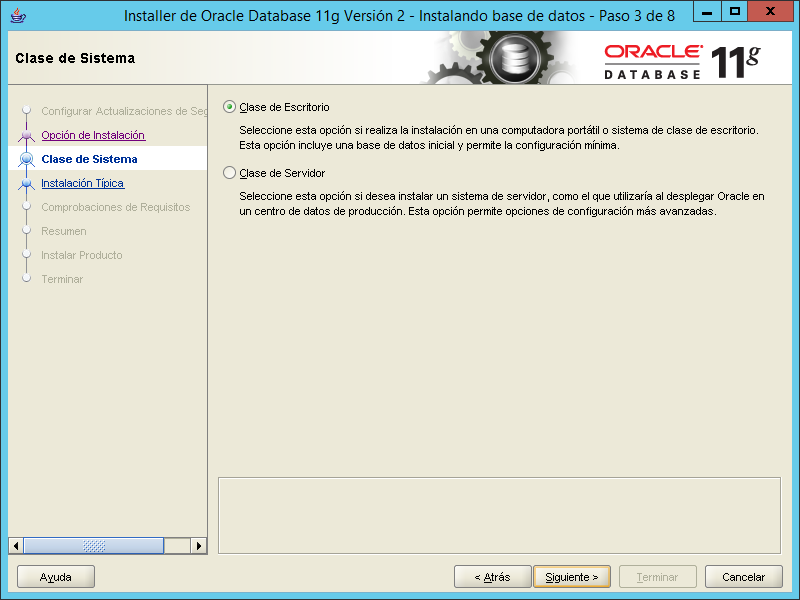
\includegraphics[width=11cm]{Imagenes/Opcion_Crear_Escritorio.png}
\end{center}

\textbf {4.3.8. Instalación Típica:} A continuación indicaremos los siguientes datos:
Directorio Base de Oracle: Ubicación del directorio raíz de Oracle
Ubicación del Software: Destino de los archivos de la instalación de Oracle.
Ubicación de Archivos de Base de Datos: Ubicación de los archivos de datos que almacenará la base de datos.
Edición de Base de Datos: Tipo de instalación, a elegir entre "Enterprise Edition", "Standar Edition", "Standard Edition One", "Personal Edition". 
Juego de Caracteres: Juego de caracteres que se asignará a la base de datos.
Nombre de la Base de Datos Global: SID que tendrá la base de datos para identificarla unívocamente de otras, por defecto "orcl".
Contraseña del Administrador: contraseña para el usuario "system" y "sys".
Confirmar Contraseña y clic en siguiente.
\begin{center}
  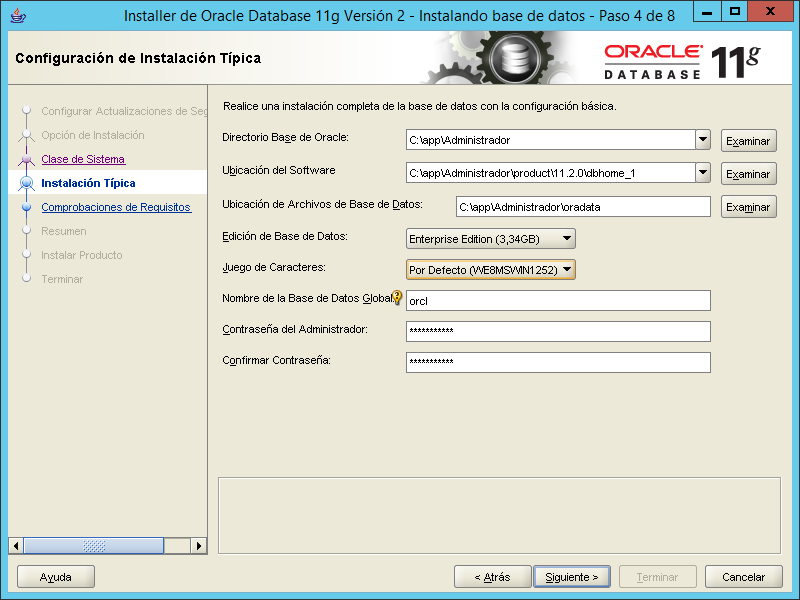
\includegraphics[width=11cm]{Imagenes/Instalacion_Tipica.png}
\end{center}
\break

\textbf {4.3.9. Resumen de la Instalación:} Se iniciará la verificación de los requisitos mínimos por parte del asistente, comprobará si la configuración y el hardware de nuestro equipo cumple con los requisitos mínimos y mostrará la ventana resumen de las opciones seleccionadas para la instalación. Clic en terminar para continuar.
\begin{center}
  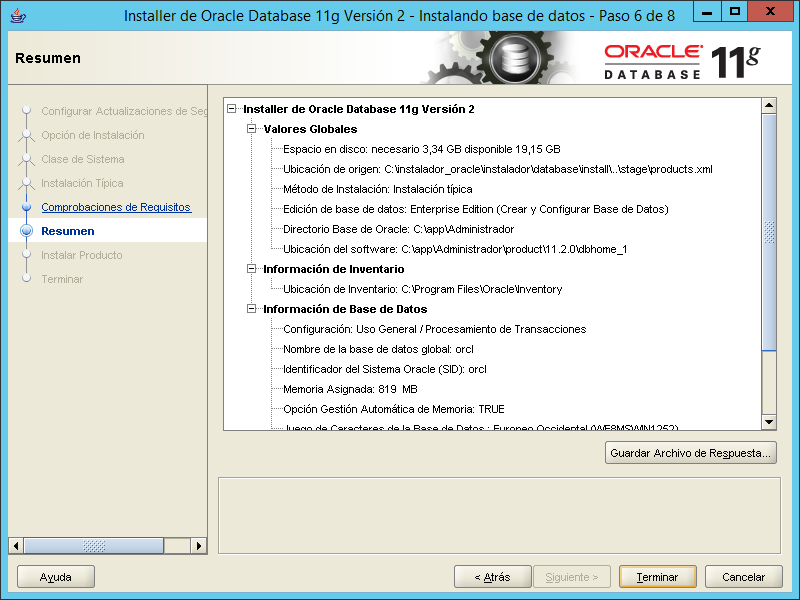
\includegraphics[width=12cm]{Imagenes/Resumen_Instalacion.png}
\end{center}

\textbf {4.3.10. Proceso de Instalación:} Este proceso demorará entre 10 a 15 minutos. El asistente nos mostrará el progreso de la instalación así como las tareas realizadas (instalación de Oracle Database, preparar sistema, copiar archivos, crear archivos de configuración, configurar Oracle Database, crear base de datos)
\begin{center}
  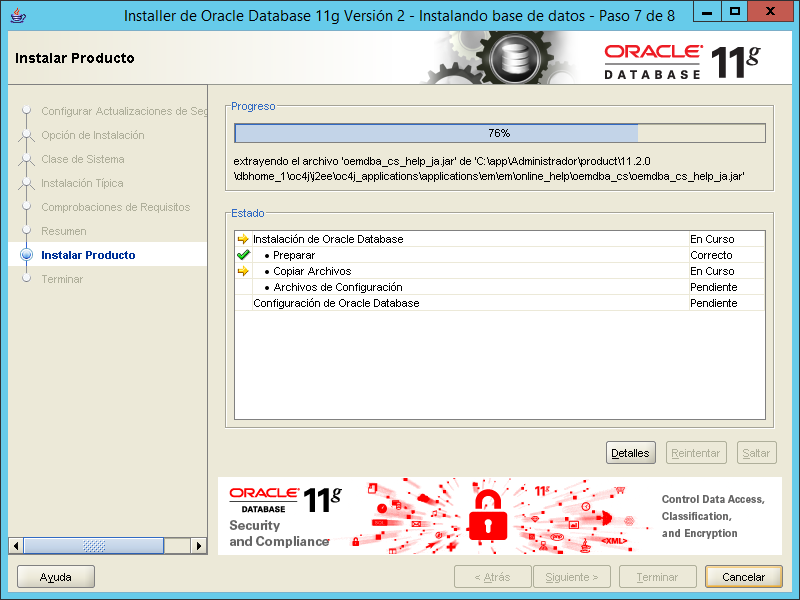
\includegraphics[width=12cm]{Imagenes/Proceso_Instalacion_Oracle.png}
\end{center}
\break

\textbf {4.3.11. Asistente de Configuración:} Al final de la instalación de Oracle se iniciará el proceso de creación de la base de datos (copia de archivos, crear e iniciar instancia de oracle):
\begin{center}
  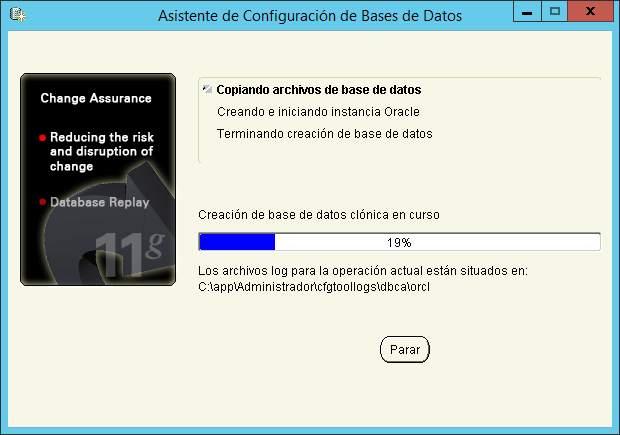
\includegraphics[width=12cm]{Imagenes/Asistente_Configuracion.png}
\end{center}

\textbf {4.3.12. Gestión de Contraseñas:} El asistente de Configuración de Bases de Datos nos mostrará la ventana desde la que podremos acceder a la gestión de contraseñas de los usuarios y en la que nos mostrará la URL de administración para acceso a Oracle Database Control, por defecto: https:\/\/localhost:1158\/em
\begin{center}
  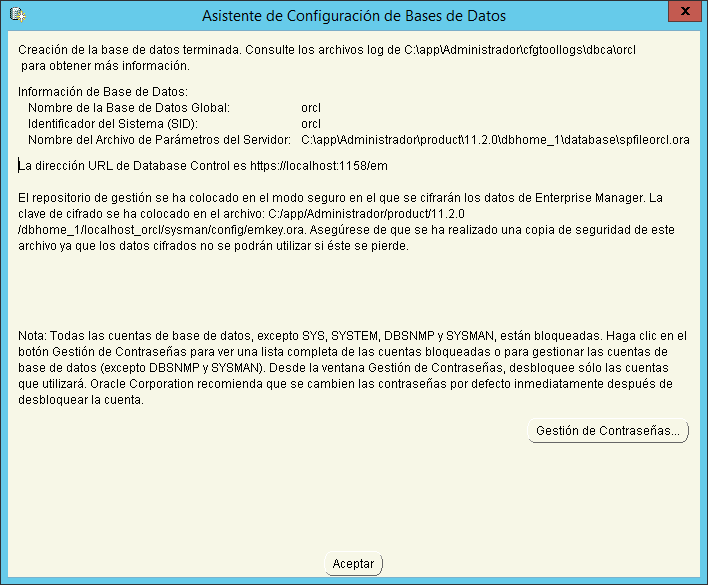
\includegraphics[width=12cm]{Imagenes/Gestion_Contrasenas.png}
\end{center}
\break

\textbf {4.3.13. Asistente de Configuración:} Por último la ventana indicando que la instalación de oracle ha sido correcta.
\begin{center}
  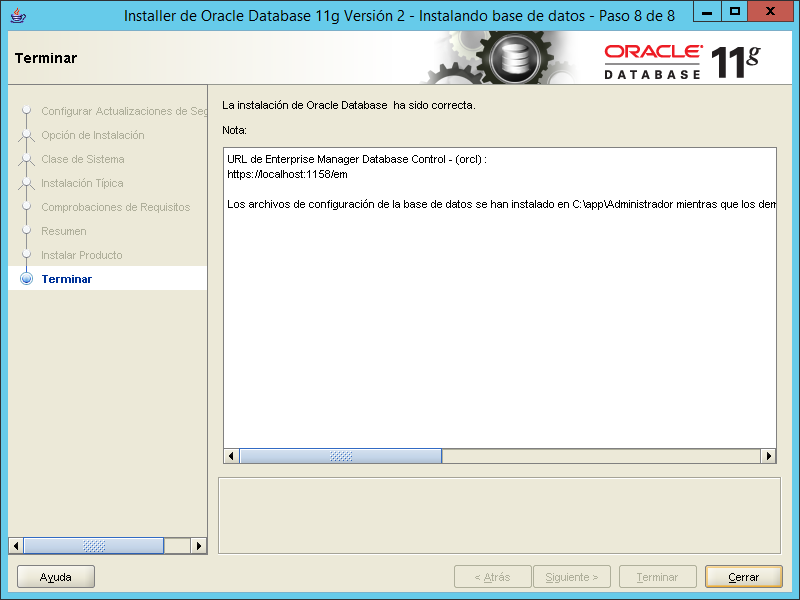
\includegraphics[width=12cm]{Imagenes/Instalacion_Correcta.png}
\end{center}

\textbf {4.3.14. Oracle DataBase:} Y listo, ahora ya podremos acceder a nuestra Base de Datos de Oracle.
\begin{center}
  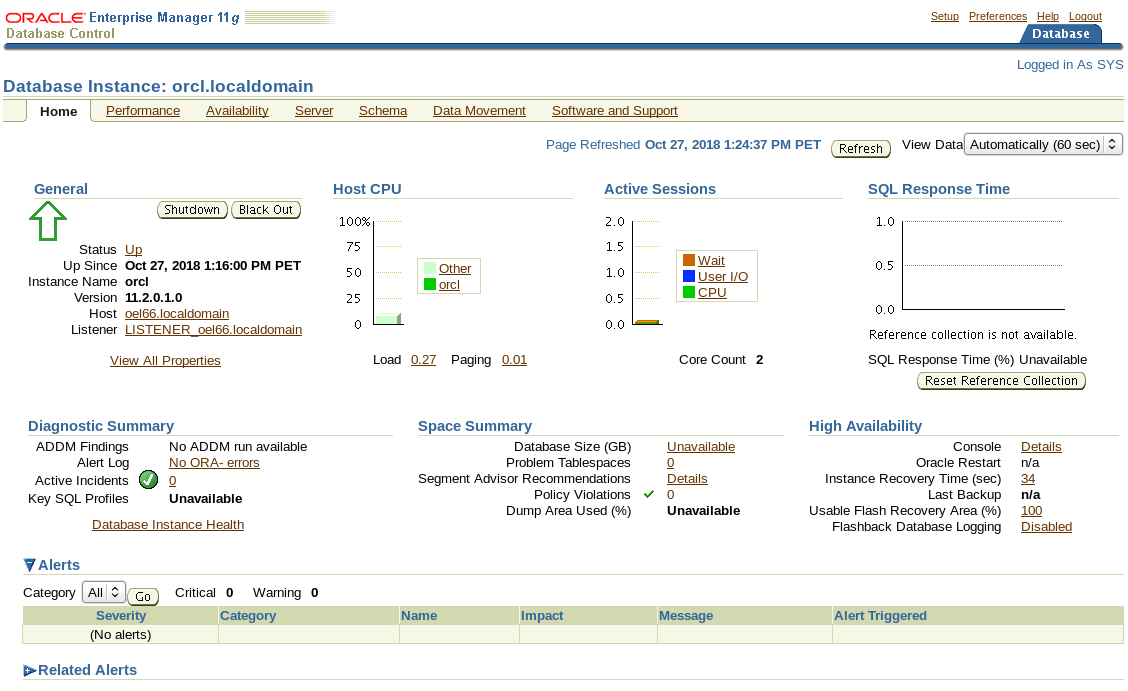
\includegraphics[width=15cm]{Imagenes/Oracle_Data_Base.png}
\end{center}
\break